\documentclass[11pt,a4paper]{article}
\usepackage[utf8]{inputenc}
\usepackage[spanish,es-tabla]{babel}
\usepackage{amsmath}
\usepackage{amsfonts}
\usepackage{amssymb}
\usepackage{graphicx}
\usepackage{natbib}
\usepackage{lineno}
\usepackage{ragged2e}
\usepackage{multicol}
\setlength\columnsep{38pt}
\usepackage{enumerate} 
\usepackage[left=2.8cm,top=2.3cm,right=2.8cm,bottom=2.3cm]{geometry} 
\usepackage{fancyhdr}
\usepackage{url}
\usepackage{float}

\begin{document}
	
	\begin{center}
		\huge \textbf{Data Warehouse VS. Data Lake} 
	\end{center}
	\vspace{\baselineskip}
	\begin{center}
		
\includegraphics[scale=0.37]{./Imagenes/logo}
	\end{center}
	\vspace{\baselineskip}
	\begin{multicols}{2}
		\small
		\begin{center}
			Nelia Escalante Marón\\
			2014049551\\
			UPT – Ingeniería de Sistemas\\
			EPIS\\
			Tacna, Perú\\
			\vspace{\baselineskip}
			Yerson Coaquira Calizaya\\
			2015053225\\
			UPT – Ingeniería de Sistemas\\  
			EPIS\\
			Tacna, Perú\\                 
			\vspace{\baselineskip}
			Flor Condori Gutierrez\\
			2015053227\\
			UPT – Ingeniería de Sistemas\\  
			EPIS\\	
			Tacna, Perú\\                 
			\columnbreak
			
			\vspace{\baselineskip}
			Christian Cespedes Medina\\
			2010036256\\
			UPT – Ingeniería de Sistemas\\  
			EPIS\\	
			Tacna, Perú\\                 
			
			\vspace{\baselineskip}
			Javier Octavio Arteaga Ramos \\
			2007028981\\
			UPT – Ingeniería de Sistemas\\  
			EPIS\\	
			Tacna, Perú\\                 
			
		\end{center}
		\normalsize			
	\end{multicols}
	\vspace{\baselineskip}
	
	\textbf{\textit{\large Resumen}}\rule[1.5mm]{5mm}{0.1mm}		
	Un lago de datos es diferente, porque almacena datos relacionales de aplicaciones de línea de negocios y datos no relacionales de aplicaciones móviles, dispositivos IoT y redes sociales. La estructura de los datos o el esquema no se define cuando se capturan los datos. Esto significa que puede almacenar todos sus datos sin un diseño cuidadoso o la necesidad de saber para qué preguntas podría necesitar respuestas en el futuro.

Seguramente han escuchado muchas veces el término de Data Warehouse; podemos definirla como una base de datos corporativa donde se integra y depura información de una o varias fuentes distintas, que luego serán procesadas y analizadas desde distintos puntos de vista con afinidad de perspectivas y grandes velocidades de respuesta.

	\rule{155mm}{0.1mm}	

	%\newpage
	\vspace{\baselineskip}

	\textbf{\textit{\large Abstract}}\rule[1.5mm]{5mm}{0.1mm} 		
	\textit{
		A lake of data is different, because it stores relational data from business line applications and non-relational data from mobile applications, IoT devices and social networks. The structure of the data or the schema is not defined when the data is captured. This means that you can store all your data without careful design or the need to know for which questions you might need answers in the future. 
Surely you have heard the term Data Warehouse many times; we can define it as a corporate database where information is integrated and filtered from one or several different sources, which will then be processed and analyzed from different points of view with affinity of perspectives and great response speeds.
	}
			
	%\rule{155mm}{0.1mm}
	
	\vspace{\baselineskip}
	
	\section{Introducción}
	
	Dependiendo de los requisitos, una organización típica requerirá tanto un almacén de datos como un lago de datos, ya que responden a diferentes necesidades y casos de uso.\\
		\\
		Un almacén de datos es una base de datos optimizada para analizar datos relacionales provenientes de sistemas transaccionales y aplicaciones de línea de negocios. La estructura de datos y el esquema se definen de antemano para optimizar las consultas SQL rápidas, donde los resultados se utilizan normalmente para informes y análisis operativos. Los datos se limpian, enriquecen y transforman para que puedan actuar como la "fuente única de verdad" en la que los usuarios pueden confiar.\\
		\\
		 Se pueden usar diferentes tipos de análisis en sus datos, como consultas SQL, análisis de big data, búsqueda de texto completo, análisis en tiempo real y aprendizaje automático para descubrir información.\\
		\\
		A medida que las organizaciones con almacenes de datos ven los beneficios de los lagos de datos, están evolucionando para que incluyan lagos de datos y habiliten diversas capacidades de consulta, casos de uso de la ciencia de datos y capacidades avanzadas para descubrir nuevos modelos de información. Gartner denomina a esta evolución como "Solución de gestión de datos para análisis" o "DMSA".
	
	\section{Marco Teórico}
	
		\subsection{Data Lake}
		
		Un data lake es un repositorio de almacenamiento que contienen una gran cantidad de datos en bruto y que se mantienen allí hasta que sea necesario. A diferencia de un data warehouse jerárquico que almacena datos en ficheros o carpetas, un data lake utiliza una arquitectura plana para almacenar los datos.\\
		\\
		Un data lake es un repositorio centralizado que le permite almacenar todos sus datos estructurados y no estructurados a cualquier escala. Puede almacenar sus datos como están, sin tener que estructurar primero los datos y ejecutar diferentes tipos de análisis, desde cuadros de mandos y visualizaciones hasta procesamiento de big data, análisis en tiempo real y aprendizaje automático para guiar mejores decisiones.
		
		\begin{figure}[H]
			\begin{center}
				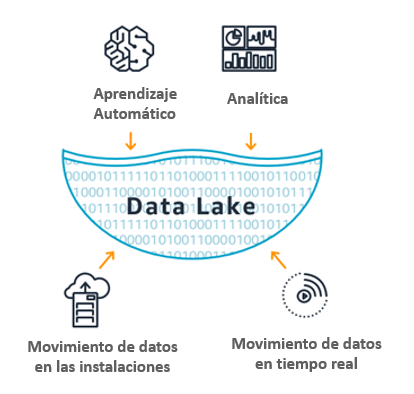
\includegraphics[scale=0.6]{./Imagenes/img01}	
				\caption{Componentes del DataLake}		
			\end{center}
		\end{figure}
	
		A cada elemento de una data lake se le asigna un identificador único y se etiqueta con un conjunto de etiquetas de metadatos extendidas. Cuando se presenta una cuestión de negocios que debe ser resuelta, podemos solicitarle al data lake los datos que estén relacionados con esa cuestión. Una vez obtenidos podemos analizar ese conjunto de datos más pequeño para ayudar a obtener una respuesta.\\
		\\
		El data lake se asocia a menudo con el almacenamiento de objetos orientado a Hadoop. En este escenario, los datos de una organización se cargan primero en la plataforma Hadoop y, a continuación, se aplican las herramientas de análisis y de minería de datos a los datos que residen en los nodos clúster de Hadoop.\\
		\\
		Al igual que con big data, el término data lake a veces se desacredita diciendo que es una simple etiqueta de marketing para un producto que soporta Hadoop. Cada vez más, sin embargo, el término está siendo aceptado como una forma de describir cualquier gran conjunto de datos en el que el esquema y los requisitos de datos no se definen hasta que los datos se consultan.\cite{DLake01:Online}
		
		\newpage

		\bibliographystyle{plain}
		\bibliography{BIBLIO}
		
	
\end{document}